\chapter{Web Services}
\label{chap:web_services}

\chapterQuote{The purpose of computing is insight, not numbers.}{\citeauthor{Hamming}}{\citeyear{Hamming}}{\cite[][Vorwort]{Hamming}}

In diesem Kapitel werden die Grundlagen zu HTTP, Dokumentbeschreibungssprachen, Beschreibungsformate für Webanwendungen und \gls{REST} erläutert, welche für das Verständnis der Arbeit wichtig sind. 
Neben \gls{XML} und  \gls{JSON} wird auch die Schemabeschreibungssprache \gls{XSD} behandelt.
Das Ende bildet die Einführung in \gls{REST} und \gls{WADL}.

\section{Adressierung}
\label{sec:addressing}

Für den Zugriff auf Dienste eines Web Services werden Adressen benötigt. Adressen im Internet sind meist nach einem bestimmten Schema aufgebaut, üblicherweise sind dies \glspl{URI}. Um Unklarheiten bei der Verwendung der Begriffe \gls{URI}, \gls{URL} und \gls{URN} im Verlauf der Arbeit zu vermeiden, werden Sie an dieser Stelle definiert.

\thesisDefinition{\gls{URI}}{
    Ein \enquote{Uniform Resource Identifier} (\gls{URI}) ist eine kompakte Zeichenkette zur Identifizierung einer abstrakten oder physischen Ressource. \ldots{} Eine Ressource ist alles was identifizierbar ist, beispielsweise elektronische Dokumente, Bilder, Dienste und Sammlungen von Ressourcen. (eigene Übersetzung von \cite{w3cURI}).
}

\thesisDefinition{\gls{URL}}{
    Der Begriff \enquote{Uniform Resource Locator} (\gls{URL}) bezieht sich auf eine Teilmenge von \glspl{URI}. \glspl{URL} identifizieren Ressourcen über den Zugriffsmechanismus, anstelle des Namens oder anderer Attribute der Ressource.
    (eigene Übersetzung von \cite{w3cURI}).   
}

\thesisDefinition{\gls{URN}}{
    Eine Teilmenge der \glspl{URI}, die sogenannten \enquote{Uniform Resource Names} (\glspl{URN}), sind global eindeutige und beständige Bezeichner für Ressourcen. Sie müssen verfügbar bleiben auch wenn die bezeichnete Ressource nicht mehr erreichbar oder vorhanden ist. \ldots{} Der Unterschied zu einer \gls{URL} besteht darin, das ihr primärer Zweck in der dauerhaften Auszeichnung einer Ressource mit einem Bezeichner besteht.
    (eigene Übersetzung von \cite{w3cURI}).
}

Beispiel \glspl{URL}:
\begin{compactitem}
    \item \texttt{http://www.spreadshirt.net/}
    \item \texttt{mailto:admin@klingt.net}
\end{compactitem}

Beispiel \glspl{URN}:
\begin{compactitem}
    \item \texttt{urn:spreadshirt:product:2648}
    \item \texttt{urn:isbn:9780131392809}
\end{compactitem}

\begin{figure}
    \centering
    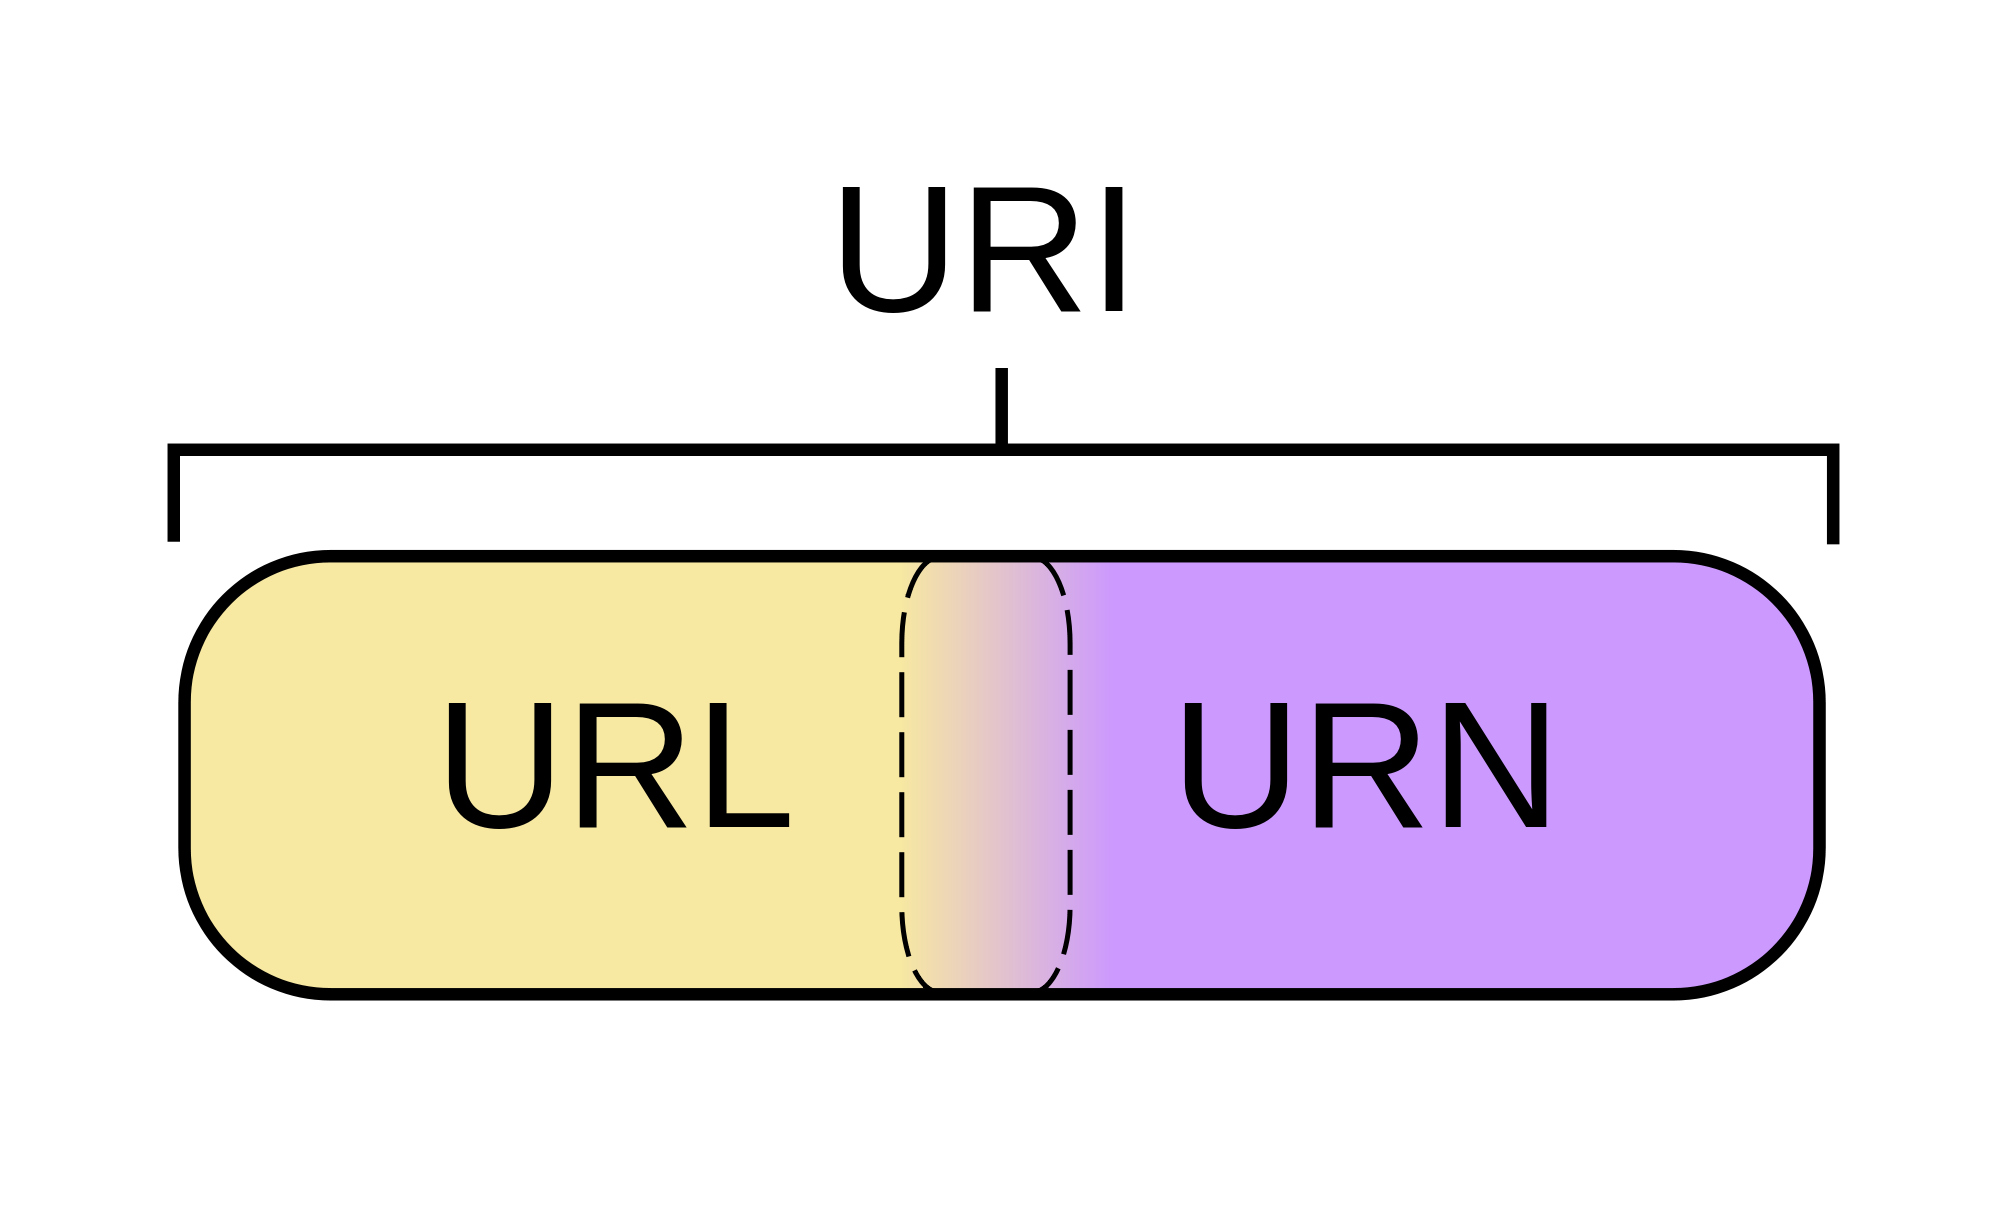
\includegraphics[width=0.4\textwidth]{resources/URI_Diagram}
    \caption{Diagramm zur Veranschaulichung der Teilmengenbeziehung zwischen den Adressierungsarten, Quelle \cite{wiki:urn}}
    \label{fig:uri_diagram}
\end{figure}

\section{HTTP}
\label{sec:http}

\thesisDefinition{HTTP}{
Das \emph{Hypertext Transfer Protocol (HTTP)} ist allgemeines und \emph{zustandsloses} Protokoll, zur Übertragung von Daten über ein Netzwerk, was durch Erweiterung seiner Anfragemethoden, Statuscodes und Header für viele unterschiedliche Anwendungen verwendet werden kann (\cite[][Abstract]{rfc2616}).
}

HTTP arbeitet auf der Anwendungsschicht\footnote{OSI-Modell Level 7} und ist somit unabhängig von dem zum Datentransport eingesetzten Protokoll. 
Über eindeutige \glspl{URI} werden HTTP-Ressourcen angesprochen. Dabei sendet ein \emph{Client} eine Anfrage (\emph{request}) und erhält daraufhin vom Server eine Antwort (\emph{response}). Anfrage und Antwort stellt dabei eine HTTP-Nachricht dar, die aus den zwei Elementen \emph{Header} und \emph{Body} besteht. Letzterer trägt die Nutzdaten und kann, je nach verwendeter HTTP-Methode, auch leer sein.

\citetitle{rfc2616} (\cite{rfc2616}) definiert einige HTTP-Methoden, wobei die gebräuchlichsten die folgenden sind:
\begin{compactitem}
    \item GET
    \item PUT
    \item POST
    \item DELETE
\end{compactitem}

%Sie gehören zur Gruppe der sogenannten \emph{CRUD}-Methoden (Create, Receive, Update, Delete) .
%\emph{Header} und \emph{Body} bilden die grundlegenden Elemente einer HTTP-Nachricht. 
Eine Nachricht kann je nach verwendeter HTTP-Methode auch nur aus einem Header bestehen.

\subsection{Header}
\label{sec:http-header}

Ein Header einer HTTP-Nachricht besteht aus einer \emph{Request Line} (erste Zeile des Headers) und einer Menge von Schlüssel-Wert Paaren. \Cref{lst:headGETrequest} zeigt einen Beispiel Header für die GET Anfrage auf die Spreadshirt-API Ressource:\\
\texttt{http://api.spreadshirt.net/api/v1/locales}.

\begin{lstlisting}[
    label=lst:headGETrequest,
    caption=HTTP-Header von GET Request auf Spreadshirt-API Ressource \texttt{http://api.spreadshirt.net/api/v1/locales}
]
GET //@\ding{202}@// /api/v1/locales //@\ding{203}@// HTTP/1.1 //@\ding{204}@//
User-Agent: curl/7.29.0 //@\ding{205}@//
Host: api.spreadshirt.net //@\ding{206}@//
Accept: */* //@\ding{207}@//
\end{lstlisting} 

\begin{compactitem}
    \item[\ding{202}] Angabe der HTTP-Methode
    \item[\ding{203}] Ressource
    \item[\ding{204}] verwendete HTTP-Version
    \item[\ding{205}] \emph{User-Agent}, Angabe zum Client-System das die Anfrage versendet
    \item[\ding{206}] \emph{Host}, Server der die Anfrage erhält und der die Ressource \ding{203} verwaltet
    \item[\ding{207}] Angabe von \emph{Content-Types} die der Client als Antwort akzeptiert, in diesem Fall eine \emph{Wildcard}, also alle Typen sind als Antwort erlaubt
\end{compactitem}

Nachfolgend die \emph{Response} auf den soeben beschrieben \emph{Request}.

\begin{lstlisting}[
    label=lst:headGETresponse,
    caption=HTTP-Header von GET Response aus Spreadshirt-API Ressource \texttt{http://api.spreadshirt.net/api/v1/locales}
]
HTTP/1.1 200 OK //@\ding{202}@//
Expires: Tue, 20 Aug 2013 19:05:25 GMT
Content-Language: en-gb
Content-Type: application/xml;charset=UTF-8 //@\ding{203}@//
X-Cache-Lookup: MISS from fish07:80
X-Server-Name: mem1
True-Client-IP: 88.79.226.66
Date: Tue, 20 Aug 2013 07:20:25 GMT
Content-Length: 1659
Connection: keep-alive
\end{lstlisting}

\begin{compactitem}
    \item[\ding{202}] \emph{Response Line}, Angabe der HTTP-Version am Anfang und danach der HTTP-Statuscode mit Kurzbeschreibung
    \item[\ding{203}] Angabe des Content-Types des Bodys der Nachricht
\end{compactitem}

Welche Einträge der Header einer HTTP-Nachricht letztendlich enhtält, ist abhängig von der Implementierung des Clients oder Servers und es können auch jederzeit eigene Einträge, die nicht in der HTTP-Spezifikation enthalten sind, hinzugefügt werden.

\subsection{Body}
\label{sec:http-body}

Der Body enthält die eigentlichen Nutzdaten. Deren Format wird mit dem \emph{Content-Type} Eintrag des Headers angegeben. \Cref{lst:bodyGETresponse} zeigt den Body der \emph{response} von \cref{lst:headGETresponse} in \gls{XML} Format (siehe \cref{sec:xml}).

\begin{lstlisting}[
    language=XML,
    label=lst:bodyGETresponse,
    caption=HTTP-Body von GET Response aus Spreadshirt-API Ressource \texttt{http://api.spreadshirt.net/api/v1/locales}
]
<?xml version="1.0" encoding="UTF-8" standalone="yes"?>
<locales xmlns:xlink="http://www.w3.org/1999/xlink" xmlns="http://api.spreadshirt.net" xlink:href="http://api.spreadshirt.net/api/v1/locales" offset="0" limit="50" count="16" sortField="default" sortOrder="default">
    <locale xlink:href="http://api.spreadshirt.net/api/v1/locales/de_DE" id="de_DE"/>
    <locale xlink:href="http://api.spreadshirt.net/api/v1/locales/fr_FR" id="fr_FR"/>
    <locale xlink:href="http://api.spreadshirt.net/api/v1/locales/en_GB" id="en_GB"/>
    <locale xlink:href="http://api.spreadshirt.net/api/v1/locales/nl_NL" id="nl_NL"/>
    <locale xlink:href="http://api.spreadshirt.net/api/v1/locales/it_IT" id="it_IT"/>
    <locale xlink:href="http://api.spreadshirt.net/api/v1/locales/no_NO" id="no_NO"/>
    <locale xlink:href="http://api.spreadshirt.net/api/v1/locales/se_SE" id="se_SE"/>
    <locale xlink:href="http://api.spreadshirt.net/api/v1/locales/es_ES" id="es_ES"/>
    <locale xlink:href="http://api.spreadshirt.net/api/v1/locales/en_EU" id="en_EU"/>
    <locale xlink:href="http://api.spreadshirt.net/api/v1/locales/en_IE" id="en_IE"/>
    <locale xlink:href="http://api.spreadshirt.net/api/v1/locales/dk_DK" id="dk_DK"/>
    <locale xlink:href="http://api.spreadshirt.net/api/v1/locales/pl_PL" id="pl_PL"/>
    <locale xlink:href="http://api.spreadshirt.net/api/v1/locales/fi_FI" id="fi_FI"/>
    <locale xlink:href="http://api.spreadshirt.net/api/v1/locales/de_AT" id="de_AT"/>
    <locale xlink:href="http://api.spreadshirt.net/api/v1/locales/fr_BE" id="fr_BE"/>
    <locale xlink:href="http://api.spreadshirt.net/api/v1/locales/nl_BE" id="nl_BE"/>
</locales>
\end{lstlisting}


\section{Dokumentbeschreibungsformate}
\label{sec:document_description_formats}

In diesem Abschnitt werden die Dokumentbeschreibungsformate \gls{XML} und \gls{JSON}, der Spreadshirt-API behandelt. Außerdem wird die Schemabeschreibungssprache \emph{XML Schema Description} eingeführt.

\subsection{XML}
\label{sec:xml}

\thesisDefinition{\textsc{Xml}}{
Die \emph{Extensible Markup Language}, kurz \gls{XML}, ist eine Auszeichnungssprache (\enquote{Markup Language}), die eine Menge von Regeln beschreibt um Dokumente in einem mensch- und maschinenlesbaren Format zu kodieren \cite{XML10Specification}.
}

Obwohl das Design von \textsc{Xml} auf Dokumente ausgerichtet ist, wird es häufig für die Darstellung von beliebigen Daten benutzt \cite{wiki:xml}, z.B. um diese für die Übertragung zu serialisieren.

\begin{lstlisting}[
        language=XML, 
        caption=Die gekürzte Antwort der \textsc{API}-Ressource \texttt{users/{userid}/designs/{designID}} als Beispiel für eine \textsc{Xml}-Datei
    ][htb]
<?xml version="1.0" encoding="UTF-8" standalone="yes"?> //@\ding{202}@//
<design xmlns:xlink="http://www.w3.org/1999/xlink" 
        xmlns="http://api.spreadshirt.net" 
        ...>//@\ding{203}@//
    <name>tape_recorder</name>
    ...
    <size unit="px">
        <width>3340.0</width>
        <height>3243.0</height>
    </size>
    <colors/>//@\ding{204}@//
    ...
    <created>
        2013-03-30T12:37:54Z //@\ding{205}@//
    </created>
    <modified>2013-04-02T11:13:02Z</modified>
</design>//@\ding{206}@//
\end{lstlisting}

Eine valide \textsc{Xml}-Datei beginnt mit der \textsc{Xml}-Deklaration \ding{202}. Diese enthält Angaben über die verwendete \textsc{Xml}-Spezifikation und die Kodierung der Datei. 
Im Gegensatz zu gewöhnlichen Tags wird dieses mit \texttt{<?} und mit \texttt{?>} beendet. 
Danach folgen beliebig viele baumartig geschachtelte \emph{Elemente} mit einem Wurzelelement \ding{203}. Die Elemente können Attribute enthalten und werden, wenn sie kein leeres Element sind \ding{204}, von einem schließenden Tag in der gleichen Stufe abgeschlossen \ding{206}. Nicht leere Zeichenketten als Kindelement sind ebenfalls erlaubt \ding{205}.

Mit Hilfe von \emph{Schemabeschreibungssprachen} (siehe \cref{sec:xmlschema}) kann der Inhalt und die Struktur eines Dokumentes festgelegt und gegen diese validiert werden. Der Begriff \textsc{Xml} Schema ist mehrdeutig und wird oft auch für eine konkrete Beschreibungssprache, die \enquote{\textsc{Xml} Schema Definition}, kurz \gls{XSD}, verwendet.


\subsection{JSON}
\label{sec:json}

\thesisDefinition{JSON}{
\emph{Javascript Object Notation}, kurz \emph{JSON}, ist ein leichtgewichtiges, textbasiertes und sprachunbhängiges Datenaustauschformat. Es ist von JavaScript abgeleitet und definiert eine kleine Menge von Formatierungsregeln für die transportable Darstellung (Serialisierung) von strukturierten Daten (nach \cite{JSONRFC}).
}

Im Gegensatz zu XML ist JSON weit weniger mächtig, es gibt z.B. keine Unterstützung für Namensräume und es wird nur eine geringe Menge an Datentypen unterstützt (siehe \cref{tab:jsonDatatypes}). 
Durch seine einfache Struktur wird aber ein deutlich geringerer \enquote{syntaktischer Overhead} erzeugt.
Mit \emph{JSON Schema} \cite{json-schema-draft} ist es möglich eine Dokumentstruktur vorzugeben und gegen diese zu validieren. 

\begin{table}[tb]
    \begin{longtable}[c]{l l}
        \toprule
        \rowcolor{lightgray}
        \textbf{primitiv}   & \textbf{strukturiert}\\
        \midrule
        Zeichenketten       & Objekte\\
        Ganz- und 
        Fließkommazahlen    & Arrays\\
        Booleans            & \\
        null                & \\
        \bottomrule
        \caption{JSON Datentypen}
        \label{tab:jsonDatatypes}
    \end{longtable}
\end{table}

Objekte werden in JSON von geschweiften- \ding{202}, Arrays hingegen von eckigen Klammern begrenzt \ding{203}. 
Objekte enthalten \emph{key-value-pairs} (Schlüssel-Wert-Paare) \ding{204}. Schlüssel sind immer Zeichenketten, die Werte dürfen von allen Typen aus \cref{tab:jsonDatatypes} sein und beliebig tief geschachtelt werden.
%
% wrapping in a minipage prevents the listings block from splitting on pagebreak
%
\begin{lstlisting}[
    language=JavaScript,
    caption=Die gekürzte Antwort der API-Ressource \emph{users/{userid}/designs/{designID}} als Beispiel für eine JSON-Datei
]
{
    "name": "tape_recorder", //@\ding{204}@//
    "description": "",
    "user": { //@\ding{202}@//
        "id": "1956580",
        "href": "http://api.spreadshirt.net/api/v1/users/1956580"
    }, //@\ding{202}@//
    "resources": [ //@\ding{203}@//
    ...
        {
            "mediaType": "png",
            "type": "preview",
            "href": "http://image.spreadshirt.net/image-server/v1/designs/15513946"
        }, 
        ...
    ], //@\ding{203}@//
    "created": "30.03.2013 12:37:54",
    ...
}
\end{lstlisting}    


% ToDo: Titel in Schemasprachen ändern?
\section{XML Schemabeschreibungssprachen (XML Schema)}
\label{sec:xmlschema}

\emph{XML Schema} bezeichnet XML-basierte Sprachen mit denen sich Elemente, Attribute und Aufbau eines XML-Dokumentes beschreiben lassen. 
Ein XML-Dokument wird als \emph{valid/gültig} gegenüber einem Schema bezeichnet, falls die Elemente und Attribute dieses Dokumentes die Bedingungen des Schemas erfüllen \cite{taxonomyXMLSchema}.
Neben XSD (siehe \cref{sec:xsd}) und RelaxNG (siehe \cref{sec:relaxng}) existieren noch weitere Schemasprachen, die hier aber aufgrund ihrer geringen Relevanz nicht behandelt werden. Die beiden hier behandelten Schemasprachen bieten den Vorteil selbst XML-Dokumente zu sein, somit können sie durch herkömmliche XML-Tools bearbeitet werden.

\subsection{XML Schema Description (XSD)}
\label{sec:xsd}

\emph{XML Schema Description} ist ein stark erweiterte Nachfolger der \emph{DTD} (Document Type Definition), derzeit spezifiert in Version 1.1 \cite{XMLSchema11Specification}. 
Die Syntax von \emph{XSD} ist XML, damit ist die Schemabeschreibung ebenfalls ein gültiges XML-Dokument. Als Dateiendung wird üblicherweise \texttt{.xsd} verwendet.

Die Hauptmerkmale von XSD sind nach \cite[Kapitel 3.2][]{taxonomyXMLSchema}
, die folgenden:
\begin{compactitem}
    \item Komplexe Typen (strukturierter Inhalt)
    \item anonyme Typen (besitzen kein \texttt{type}-Attribut)
    \item Modellgruppen
    \item Ableitung durch Erweiterung oder Einschränkung (\enquote{derivation by extension/restriction})
    \item Definition von abstrakten Typen
    \item Integritätsbedingungen (\enquote{integrity constraints}):\\
        \emph{unique}, \emph{keys} und \emph{keyref}, dies entspricht den \emph{unique-}, \emph{primary-} und \emph{foreign}-keys aus dem Bereich der Datenbanken        
\end{compactitem}

\begin{lstlisting}[
    language=XML,
    caption=Beginn der XSD-Datei für die Spreadshirt-API,
    label=lst:xsdIntro
    ]
<?xml version="1.0" encoding="UTF-8" standalone="yes"?> //@\ding{202}@//
<xs:schema xmlns:xs="http://www.w3.org/2001/XMLSchema"  targetNamespace="http://api.spreadshirt.net" version="1.0" elementFormDefault="qualified"> //@\ding{203}@//
    <xs:import namespace="http://www.w3.org/1999/xlink" schemaLocation="xlink.xsd"/> //@\ding{204}@//
    ...
\end{lstlisting}

Eine XSD-Datei beginnt wie jede XML-Datei mit der XML-Deklaration \ding{202}.

Das Wurzelelement der Schemadefinition zeigt \ding{203}. 
Das Attribut \emph{xmlns:xs= "http://www.w3.org/2001/XMLSchema"} führt den Namespace-Prefix \emph{xs} ein und gibt außerdem an, dass die Elemente und vordefinierten Datentypen (siehe \cref{fig:xsddatatypes}) aus dem Namensraum \emph{http://www.w3.org/2001/XMLSchema} verwendet werden. Durch das Attribut \emph{targetNamespace} wird der Namensraum der Elemente festgelegt, die in dieser Schemadefinition definiert werden. \emph{Version} gibt die XSD-Version an.
Der Wert des Attributs \emph{elementFormDefault} gibt an, ob Elemente des Schemas den \emph{targetNamespace} explizit angeben müssen (\enquote{qualified}) oder ob dies implizit geschieht (\enquote{unqualified}), die Angabe ist optional.

Externe Schemadefinitionen lassen sich unter Angabe des Namensraumes und einer \gls{URI} zu der XSD-Datei einbinden \ding{204}.

XML Schema Description erlaubt die Definition von simplen Typen (\enquote{SimpleType}) und Typen mit strukturiertem Inhalt (\enquote{ComplexType}).

\begin{lstlisting}[
    language=XML,
    caption=Beispiel für einen SimpleType anhand des Type \enquote{unit} der Spreadshirt-API,
    label=lst:xsdExampleUnit
]
<xs:simpleType name="unit">
    <xs:restriction base="xs:string"> //@\ding{202}@//
        <xs:enumeration value="mm"/> //@\ding{203}@//
        <xs:enumeration value="px"/> //@\ding{203}@//
    </xs:restriction>
</xs:simpleType>
\end{lstlisting}

\emph{SimpleType}-Definitionen dienen zur Beschreibung einfacher Typen wie \emph{Enumeratoren}, oder \emph{Listen} für Daten eines primitiven Typs. Ein Beispiel für die Definition eines Enumerators durch einen SimpleType zeigt \Cref{lst:xsdExampleUnit}. Der Basisdatentyp des Enumerators wird dabei durch die Angabe des Attributs \emph{base} \ding{202} festgelegt. Zuordnung von Werten zu dem Enumerator zeigt \ding{203}.

Durch einen SimpleType definierte Listen sind durch Leerzeichen separierte Strings, sie werden meist für den Wert eines Attributes einer XML-Datei verwendet. 

\begin{lstlisting}[
    language=XML,
    caption=Beispiel für einen Listentyp definiert duch einen SimpleType,
    label=lst:xsdListExample    
]
<xs:simpleType name=colors>
    <xs:list itemType="xs:string"/>
</xs:simpleType>
\end{lstlisting}

\begin{lstlisting}[
    language=XML,
    caption=Beispielinstanz für Typ aus \Cref{lst:xsdListExample},
    label=lst:xsdListExampleInstance
]
<test>red green blue</test>}
\end{lstlisting}

Die Definition eines strukturierten Typs zeigt \Cref{lst:xsdExampleAbstractList}.

\begin{lstlisting}[
    language=XML, 
    caption=Beispiel für eine Schemabeschreibung mit XSD anhand des \enquote{abstractList}-Typs der Spreadshirt-API,
    label=lst:xsdExampleAbstractList
    ]
<xs:complexType name="abstractList" abstract="true"> //@\ding{202}@//
    <xs:sequence> //@\ding{203}@//
        <xs:element minOccurs="0" //@\ding{204}@// name="facets"> //@\ding{205}@//
            <xs:complexType> //@\ding{206}@//
                <xs:sequence>
                    <xs:element xmlns:tns="http://api.spreadshirt.net" minOccurs="0" maxOccurs="unbounded" ref="tns:facet" //@\ding{207}@// />
                </xs:sequence>
            </xs:complexType>
        </xs:element>
    </xs:sequence>
    <xs:attribute xmlns:xlink="http://www.w3.org/1999/xlink" ref="xlink:href"/> //@\ding{208}@//
    <xs:attribute type="xs:long" name="offset"/> //@\ding{209}@//
    <xs:attribute type="xs:string" name="query"/>        
    ...
</xs:complexType>
\end{lstlisting}

Das \emph{ComplexType}-Tag \ding{202} umschließt die Definiton des strukturierten Typs. XML Schema Description erlaubt das definieren von abstrakten Typen, nur Ableitungen davon dürfen als Instanzen in einem Dokument auftreten. Abgeleitete Typen dürfen dabei den abstrakten Typ \emph{erweitern} o. \emph{einschränken} (\enquote{derivation by extension/restriction}).

Mit \emph{Reihenfolgeindikatoren} \ding{203} kann die Ordnung von Elementen festgelegt werden. Elemente unterhalb eines \emph{Sequence}-Tags dürfen nur in der Abfolge auftreten in der sie unterhalb des Sequence-Tag definiert worden sind. Das \emph{All}-Tag \ding{205} hingegen erlaubt das auftreten ohne festgelegte Reihenfolge. Der Reihenfolgeindikator \emph{Choice} erlaubt das auftreten nur eines der Elemente die unterhalb dieses Tags vorkommen.

Durch die optionale Angabe von \emph{Häufigkeitsindikatoren} \ding{204} kann festgelegt werden wie oft ein Element an der definierten Stelle vorkommen darf. Entfällt dies, entspricht der Wert von \emph{min-, maxOccurs} "1", das heisst das Element darf genau einmal an dieser Stelle vorkommen.

Elemente einer XML-Datei werden durch das gleichnamige \emph{Element} \ding{205} im XSD definiert. Ein Element benötigt die Angabe eines Namens und Typs. Die Angabe des Typs kann dabei als Referenz auf die Typdefinition \ding{207} oder als Definition unterhalb des Element-Tags erfolgen \ding{206}.

Attribute eines XML-Tags werden durch das \emph{Attribute}-Element definiert. Dies geschieht durch Angabe von Name und Typ \ding{208} oder durch eine Referenz auf eine Attributdefinition \ding{207}.

Referenzen haben die Form \emph{Namensraumbezeicher}:\emph{Elementname}. Wobei mit Elementname jedes Element der Schemabeschreibung gemeint ist, welches ein \emph{name}-Attribut besitzt. Der konkrete Namensraum eines solchen Bezeichners wird vorher mit der Angabe eines Attributes in dieser Form eingeführt:

\[  
    \underbrace{\texttt{xmlns:tns}}_{\tiny \text{XML-Namespace:Namensraumbezeichner}}\texttt{=}\underbrace{\texttt{"http://api.spreadshirt.net"}}_{\tiny \text{Konkreter Namensraum}}
\]

%
% todo: xml schema genauer beschreiben, relaxng entfernen --: Beispiel fuer Instanz und Definition des Typs!
%

\begin{sidewaysfigure}
    \centering
    \tikzstyle{blueBox}=[
        rectangle,
        fill={blue!15},
        draw,
        font=\sffamily
    ]      
    \tikzstyle{grayBox}=[
        rectangle,
        fill=lightgray,
        text=black,
        font=\sffamily,
        draw
    ]
    \tikzstyle{violetBox}=[
        rectangle,
        fill=violet,
        text=white,
        font=\sffamily,
        draw
    ]
    \tikzstyle{greenBox}=[
        rectangle,
        fill=green!50,
        text=black,
        font=\sffamily,
        draw
    ]
    \tikzstyle{derivedFromList}=[
        dashed,
        cyan
    ]
    \resizebox{\textheight}{!}{
            \input{tikz_pgf/xsd_predefined_types}
    }
    \vspace{\baselineskip}\\
    \resizebox{0.5\textheight}{!}{
            \input{tikz_pgf/xsd_predefined_types_legend}
    }        
    \caption{vordefinierte XSD Datentypen nach \cite{XMLSchema11Specification} Kapitel 3}
    \label{fig:xsddatatypes}
\end{sidewaysfigure}

\subsection{RelaxNG}
\label{sec:relaxng}

% Wikipedia, satz abändern
Ebenso wie XSD (siehe \cref{sec:xsd}) ist die \emph{Regular Language Description for XML New Generation} eine XML-Schemasprache zur Definition der Struktur von XML-Dokumenten. 
Schemas werden in \emph{RelaxNG} durch XML-Syntax oder eine eigene, kompaktere nicht-XML Syntax formuliert. Ebenso wie bei \emph{XML Schema} werden Namespaces unterstützt. RelaxNG Schemabeschreibungen verwenden meist \texttt{.rng} als Dateiendung.

Unterschiede zu XML Schema:
\begin{compactitem}
    \item Unterstützung von ungeordneten Inhalten
    \item kompaktere nicht-XML Syntax
    \item \emph{nichtdeterministisches} oder auch \emph{mehrdeutiges} Inhaltsmodell \cite[Kapitel 16]{RelaxNGVlist}    
    % Beispiel von http://pike.psu.edu/publications/toit05.pdf Seite 17
\end{compactitem}

\begin{lstlisting}[
    language=XML, 
    caption=Minimalbeispiel für eine Schemadefinition in RelaxNG, 
    label=minimalRelaxNG]
<?xml version="1.0" encoding="utf-8"?>
<grammar 
    xmlns="http://relaxng.org/ns/structure/1.0"
    ns="myNamespace">
    <start>
        <ref name="product"/>
    </start>
    <define name="product">
        <oneOrMore>
            <element name="name"/>
                <text/>
            </element>
            <element name="price"/>
                <text/>
            </element>
            <ref name="description"/>
        </oneOrMore>
    </define>
    <define name="description">
        <oneOrMore>
            <element name="title">
                <text/>
            </element>
            <element name="content">
                <text/>
            </element>
        </oneOrMore>
    </define>
</grammar>
\end{lstlisting}



\section{RESTful Web Service}
\label{sec:rest}

\emph{Representational State Transfer} (deutsch: \enquote{Gegenständlicher Zustandstransfer}) ist ein Softwarearchitekturstil für Webanwendungen, welcher von Roy Fielding\footnote{Roy Thomas Fielding, geboren 1965, ist einer der Hauptautoren der HTTP-Spezifikation} in seiner Dissertation aus dem Jahre 2000  beschrieben wurde \cite[Kapitel 5][95 ff.]{fieldingDissertation}. 

Als \gls{RESTful} bezeichnet man dabei eine Webanwendung die den Prinzipien von \gls{REST} entspricht. 

% Diesen Part über die Grundprinzipien verschieben
\subsection{Elemente von REST}

Im folgenden werden die Grundbausteine einer REST-Anwendung erläutert. \Cref{sec:RESTcomponents} beschreibt die Komponenten, die an einer Aktion auf einer \emph{Ressource} beteiligt sind. Dieser Abschnitt basiert auf Kapitel 5.2 von \cite[][S. 86 ff.]{fieldingDissertation}.

\subsubsection{Ressource}

Eine Ressource stellt die wichtigste Abstraktion von Information im REST-Modell dar. Fielding definiert eine \emph{ressource} wie folgt:

\thesisquote{Any information that can be named can be a resource: a document or image, [\ldots]. A resource is a conceptual mapping
to a set of entities, not the entity that corresponds to the mapping at any particular point in
time.}

Eine Ressource kann somit alle Konzepte abbilden die sich über einen Bezeichner referenzieren lassen. Dies können konkrete Dokumente, aber auch Dienste oder sogar Sammlungen von Ressourcen sein.
Außerdem identifiziert ein Ressourcenbezeichner, meist eine \emph{URI} (siehe \cref{sec:unambigiousidentification}), immer dieselbe Ressource, nicht aber deren Wert oder Zustand.

\subsubsection{Repräsentation}

Eine Repräsentation (\emph{representation}) stellt den aktuellen oder den gewünschten Zustand einer Ressource dar. Das Format der Repräsentation ist dabei unabhängig von dem der Ressource, siehe \cref{sec:representationofresources}.
Aktionen mit Komponenten einer REST-API werden durch den Austausch von solchen Repräsentationen durchgeführt.

Im Allgemeinen wird unter einer Repräsentation nur eine Folge von Bytes verstanden, inklusive \emph{Metainformationen} welche den Inhalt der Bytefolge klassifiziert, sowie \emph{Kontrolldaten} die die gewünschte Aktion oder die Bedeutung der Anfrage beschreiben. Letztere sind meist HTTP-Header-Felder\footnote{für die HTTP-Header-Definitionen siehe \url{http://www.w3.org/Protocols/rfc2616/rfc2616-sec14.html\#sec14.43}}, bspw. um das Cachingverhalten zu ändern.

\begin{minipage}{\textwidth}
    \begin{lstlisting}[
        language=XML,
        caption=Beispiel zu Metainformationen für REST-Repräsentation aus WADL-Datei der Spreadshirt-API,
        label=lst:metainformationREST
        ]
    ...
    <response>
        <representation xmlns:sns="http://api.spreadshirt.net",
            element="sns:productTypes" status="200", //@{\ding{202}}@//
            mediaType="application/xml"> //@{\ding{203}@//
            <doc title="Success"/>
        </representation>
        ...
    </response>
    \end{lstlisting}
\end{minipage}

Ein Beispiel für eine solche Angabe von Metainformationen ist in \Cref{lst:metainformationREST} zu finden, \ding{202} zeigt dies in Form einer \emph{Typangabe} und \ding{203} eines \emph{mediaType}-Attributes.

\subsubsection{Konnektoren}

Konnektoren stellen eine Schnittstelle für die Kommunikation mit Komponenten der REST-Webanwendung dar. Aktionen auf Ressourcen und der Austausch von Repräsentationen finden über diese Schnittstellen statt. Der Konnektor bildet die Parameter der Schnittstelle auf das gewünschte Protokoll ab.

Eingangsparameter\footnote{\textperiodcentered optionaler Parameter}:
\begin{compactitem}
    \item Anfrage-Kontrolldaten
    \item Ressourcenidentifizierung (Ressourcenbezeichner)
    \item[\textperiodcentered] Repräsentation der Ressource
\end{compactitem}
Ausgangsparameter:
\begin{compactitem}
    \item Antwort-Kontrolldaten
    \item[\textperiodcentered] Metainformationen
    \item[\textperiodcentered] Repräsentation der Ressource
\end{compactitem}

\Cref{tab:RESTconnectors} listet Beispiele für Konnektoren auf.

\begin{table}[tb]
    \begin{longtable}[c]{l l}
        \toprule
        \rowcolor{lightgray}
        \textbf{Konnektor}   & \textbf{Beispiel}\\
        \midrule
        client      & libwww\\
        server      & libwww, Apache HTTP-Server API\\
        cache       & browser cache, Akamai\\
        resolver    & bind\\
        tunnel      & SOCKS\\
        \bottomrule
        \caption{Beispiele für Konnektoren nach \cite{fieldingDissertation}}
        \label{tab:RESTconnectors}
    \end{longtable}
\end{table}       

\subsubsection{Komponenten}
\label{sec:RESTcomponents}

\begin{description}
    \item[Ursprungsserver] 
        Serverseitiger Konnektor der den Namespace der angeforderten Ressource verwaltet. Er ist die einzige Quelle für Repräsentationen, sowie der endgültige Empfänger von Änderungsanfragen an seine Ressourcen. (siehe \cref{sec:unambigiousidentification}).
    \item[Proxy] Zwischenkomponente die explizit vom Client verwendet kann, aus Sicherheits-, Performance- oder Kompatibilitätsgründen.
    \item[Gateway] Dient als Schnittstelle zwischen Client- und Servernetzwerk, kann zusätzlich aus den gleichen Gründen wie der Proxy verwendet werden. Konträr zum Proxy kann der Client aber nicht entscheiden ob er einen Gateway nutzen möchte.
    \item[User Client] 
        Ein clientseitiger \emph{Konnektor}, der die Anfrage an die API startet und einziger Empfänger der Antwort ist. In den meisten Fällen ist dies einfach ein \emph{Webbrowser}.
\end{description}

\subsection{REST-Prinzipien}

Die fünf Grundlegenden REST-Prinzipien, nach \cite[11 ff.]{Tilkov09}:
\begin{compactitem}
    \item Ressourcen mit eindeutiger Indentifikation
    \item Verknüpfungen / Hypermedia
    \item Standartmethoden (siehe \cref{sec:standardmethods})
    \item unterschiedliche Repräsentationen
    \item statuslose Kommunikation
\end{compactitem}

\subsubsection{Eindeutige Identifikation}
\label{sec:unambigiousidentification}

Um eine \emph{eindeutige Identifikation} zu erreichen, wird jeder Ressource eine \gls{URI} vergeben. Dadurch ist es möglich zu jeder verfügbaren Ressource einen Link zu setzen. 
Nachfolgend eine Beispiel-URI, um den Artikel 42 aus dem Warenkorb 84 anzusprechen:
\[
    \underbrace{http://api.spreadshirt.net/api/v1/}_{Basis-URL}\underbrace{\overbrace{baskets/84}^{Warenkorb}\overbrace{/item/42}^{Artikel}}_{Ressource}
    \label{RESTexampleURL}
\]

\subsubsection{Hypermedia}
\label{sec:hypermedia}

Innerhalb einer Ressource kann auf weitere verlinkt werden (\emph{Hypermedia}). Als Nebeneffekt der eindeutigen Identifikation durch \glspl{URI} sind diese auch außerhalb des Kontextes der aktuellen Anwendung gültig. 

Das Folgen eines Links entspricht dabei einer Zustandsänderung innerhalb der Anwendung.
Die vorhandenen Verknüpfungen legen fest welche Zustandsübergänge  erlaubt sind.

\subsubsection{Standardmethoden}
\label{sec:standardmethods}

Durch die Nutzung von \emph{Standardmethoden} ist abgesichert das eine Anwendung mit den Ressourcen arbeiten kann, vorausgesetzt sie unterstützt diese. 

\gls{REST} ist nicht auf HTTP beschränkt, praktisch alle REST-APIs nutzen aber dieses Protokoll. HTTP umfasst dabei folgende Methoden\footnote{Kapitel 9 des HTTP 1.1 RFC2616 beschreibt diese inklusive \emph{TRACE} und \emph{CONNECT} umfassend \cite{HTTP11RFC}}:
\begin{compactitem}
    \item GET
    \item PUT
    \item POST
    \item DELETE
    \item HEAD
    \item OPTIONS
\end{compactitem}

Alle bis auf \emph{POST} und \emph{OPTIONS} sind \emph{idempotent} (\cite{HTTP11RFC} Kapitel 9), d.h. eine hintereinander Ausführung der Methode führt zu demselben Ergebnis wie ein einzelner Aufruf. Dies bedeutet das sich ein \emph{RESTful Web Service} serverseitig ebenso verhalten muss.

\subsubsection{Repräsentationen von Ressourcen}
\label{sec:representationofresources}

Die Repräsentation sollte unabhängig von der Ressource sein, um die Darstellung gegebenenfalls für den Client anzupassen. 
Die Client-Anwendung kann dadurch mittels \emph{Query-Parameter} oder als Information im \emph{HTTP-Header} das gewünschte Format angeben und erhält die entsprechend formatierte Antwort.
Anhand des \emph{Content-Type} Feldes aus dem HTTP-Header kann der Client das Format der Antwort überprüfen, für \gls{JSON} lautet dies bspw. \texttt{application/json}.

\subsubsection{Statuslose Kommunikation}
\label{sec:stateless_communication}

Es soll kein Sitzungsstatus (\emph{session-state}) vom Server gespeichert werden, d.h. jede Anfrage des Client muss alle Informationen enthalten, die nötig sind um diese serverseitig verarbeiten zu können. Der Sitzungstatus wird dabei vollständig vom Client gehalten. 
Diese Restriktion führt zu einigen Vorteilen:
\begin{compactitem}
    \item Verringerung der Kopplung zwischen Client und Server
    \item zwei aufeinanderfolgende Anfragen können von unterschiedlichen Serverinstanzen beantwortet werden
    \item[$\hookrightarrow$] verbesserte Skalierbarkeit
\end{compactitem}

Daraus resultiert eine erhöhte Netzwerklast, da die Statusinformationen bei jeder Anfrage mitgesendet werden müssen.


\section{WADL}
\label{sec:wadl}

Die \emph{Web Application Description Language} (kurz \gls{WADL}) ist eine maschinenlesbare Beschreibung einer \gls{HTTP}-basierten Webanwendung einschließlich einer Menge von \gls{XML} Schematas \cite{hadleyWADL}.
Die aktuelle Revision ist vom \citedate{WADLcurrent} \cite{WADLcurrent}. Im weiteren beziehe ich mich aber auf die in der Spreadshirt-\gls{API} verwendeten Version, datiert am 9. November 2006. Die Unterschiede zwischen beiden Revisionen können unter \cite{WADLchanges} nachvollzogen werden.

Die Beschreibung eines Webservices durch \gls{WADL} besteht nach \cite{hadleyWADL} im groben aus den folgenden vier Bestandteilen (eigene Übersetzung):
\begin{description}
     \item[Menge von Ressourcen] Analog einer Sitemap, also die Übersicht aller verfügbaren Ressourcen
     \item[Beziehungen zwischen Ressourcen] die kausale und referentielle Verknüpfung zwischen Ressourcen
     \item[Methoden die auf Ressourcen angewendet werden können] die von der jeweiligen Ressource unterstützten [\gls{HTTP}]-Methoden, deren Ein- und Ausgabe, sowie die unterstützten Formate
     \item[Ressourcenrepräsentationen] die unterstützten \gls{MIME}-Typen und verwendeten Datenschemata (\cref{sec:xsd})
\end{description} 

\newpage

\begin{minipage}{\textwidth}
\begin{lstlisting}[language=XML, caption={Beispielaufbau einer \gls{WADL}-Datei anhand der Spreadshirt-\gls{API} Beschreibung}, label=lst:wadlstructure, name=wadlstructure]
<?xml version="1.0" encoding="UTF-8" standalone="yes"?> //@\ding{202}@//
<application xmlns="http://research.sun.com/wadl/2006/10"> //@\ding{203}@//
    <grammars> //@\ding{204}@//
        <include href="http://api.spreadshirt.net/api/v1/metaData/api.xsd">
            <doc>Catalog XML Schema.</doc>
        </include>
        ...
    </grammars>
    <resources base="http://api.spreadshirt.net/api/v1/"> //@\ding{205}@//
        <resource path="users/{userId}"> //@\ding{206}@//
            <doc>Return user data.</doc>
            <method name="GET"> //@\ding{207}@//
                <doc>...</doc>
                <request> //@\ding{208}@//
                    <param 
                        xmlns:xsd="http://www.w3.org/2001/XMLSchema" 
                        name="mediaType" 
                        style="query" 
                        type="xsd:string">
                    <doc>...</doc>
                    </param>
                    ...
                </request>
                <response> //@\ding{209}@//
                    <representation 
                        xmlns:sns="http://api.spreadshirt.net"
                        element="sns:user" 
                        status="200" 
                        mediaType="application/xml">
                    <doc title="Success"/>
                    </representation>
                    <fault status="500" mediaType="text/plain">
                        <doc title="Internal Server Error"/>
                    </fault>
                    ...
                    }
                ...
</application>
\end{lstlisting}
\end{minipage}

Die Datei beginnt mit der Angabe der \gls{XML}-Deklaration \ding{202}.
Die Attribute des Wurzelknotens \texttt{<application>} enthalten \emph{namespace} Definitionen, u. a. auch den der verwendeten \gls{WADL}-Spezifikation \ding{203}.
Innerhalb des \texttt{<grammars>} Elements werden die benutzten \gls{XML} Schemas angegeben \ding{204}. 
Um die Ressourcen der Webanwendung ansprechen zu können, wird noch die Angabe der Basisadresse benötigt \ding{205}. 
Innerhalb des \texttt{<resources>} Elements findet sich die Beschreibung der einzelnen Ressourcen. Diese sind gekennzeichnet durch eine zur Basisadresse relativen \gls{URI} \ding{206}. In \texttt{\{\ldots\}} eingeschlossene Teile einer \gls{URI} werden durch den Wert des gleichnamigen \emph{request} Parameters ersetzt um die \gls{URI} zu bilden (generative \glspl{URI}).
Im Folgenden werden die von der Ressource unterstützten \gls{HTTP}-Methoden beschrieben \ding{207}, deren Anfrageparameter \texttt{<request>} \ding{208} sowie die möglichen Ausgaben der jeweiligen Methode \texttt{<response>} \ding{209}.

Die Dokumentations-Tags \texttt{<doc>} sind für alle \gls{XML}-Elemente optional.
Um das Listing nicht unnötig zu verlängern, wurden die schließenden \emph{Tags} weggelassen.

\Cref{fig:wadlstructure} zeigt die baumartige Struktur einer \gls{WADL}-Datei. Die Kanten enthalten Informationen über Kardinalität oder die Form des Elements (Definition/Referenz). Innerhalb der Elemente sind deren Attribute aufgelistet, oder \enquote{\ldots} falls diese schon aufgelistet wurden.

\newpage

\begin{figure}
    \centering
    \resizebox{!}{1.1\textwidth}{
        \begin{tikzpicture}[
    level 1/.style={
        font=\large,
        sibling distance=4cm,
        level distance=5cm
    },
    level 2/.style={
        font=\normalsize,
        level distance=4.5cm,
        sibling distance=7cm
    },
    level 3/.style={
        font=\small,
        level distance=4cm,
        sibling distance=2cm
    },
    level 4/.style={
        level distance=3cm,
        sibling distance=2cm
    }
    edge from parent/.style={
        draw=black,
        shorten >=5mm,
        shorten <=5mm
    },
    edgeText/.style={
        sloped,
        near end,
        above
    },    
    centeredEdgeText/.style={
        sloped,
        above
    },                
    every two node part/.style={
        color=magenta,
        font=\scriptsize,
        align=left
    },
    element/.style={
        rectangle,
        rounded corners,
        draw=gray,
        very thick
    },
    splitElement/.style={
        rectangle,
        rounded corners,
        draw=gray,
        very thick,
        rectangle split, 
        rectangle split parts=2
    }
]
\node {\Large \textbf{application}}
child {
    node [splitElement] {
        doc
        \nodepart{two}
        xml:lang\\
        title
    }
    edge from parent node[edgeText] {0..*};
}
child {
    node [element] {grammars}
    child [level distance = 2.5cm] {
        node [splitElement] {
            include
            \nodepart{two}
            href
        }
        edge from parent node[edgeText] {0..*};
    }
    edge from parent node[edgeText] {0..1};
}
child {
    node [splitElement] {
        resources
        \nodepart{two}
        base
        }
    child [sibling distance=6cm] {
        node [splitElement] {
            resource\_type
            \nodepart{two}
            id
        }
        child {
            node [splitElement] {
                doc
                \nodepart{two}
                \ldots
            }
            edge from parent node [edgeText] {0..*};
        }
        child {
            node [splitElement] {
                param
                \nodepart{two}
                id\\
                name\\
                style\\
                type\\
                default\\
                path\\
                required\\
                repeating\\
                fixed
            }
            child {
                node [splitElement] {
                    option
                    \nodepart{two}
                    value
                }
                child {
                    node [splitElement] {
                        doc
                        \nodepart{two}
                        \ldots
                    }
                    edge from parent node [edgeText] {0..*};
                }
            }
            child {
                node [splitElement] {
                    link
                    \nodepart{two}
                    resource\_type\\
                    rel\\
                    rev\\
                    location\\
                    index
                } 
                edge from parent node [edgeText] {0..*};
            }
            edge from parent node [edgeText] {0..*};
        }
        child {
            node [splitElement] {
                method
                \nodepart{two}
                \ldots
            }
            edge from parent node [edgeText] {0..*};
        }
        edge from parent node [edgeText] {0..*};
    }
    child {
        node [splitElement] {
            resource
            \nodepart{two}
            id\\
            path\\
            type\\
            queryType
            }
        child {
            node [splitElement] {
                doc
                \nodepart{two}
                \ldots
            }
            edge from parent node[edgeText] {0..*};       
        }
        child  {
            node [splitElement] {
                param
                \nodepart{two}
                \ldots
                }
            edge from parent node[edgeText] {0..*};                    
        }
        child {
            node [splitElement] {
                method
                \nodepart{two}
                \ldots
            }
            edge from parent node[edgeText] {0..*};                    
        }
        child {
            node [splitElement] {
                resource
                \nodepart{two}
                \ldots
            }
            edge from parent node[edgeText] {0..*};
        }
        edge from parent node [edgeText] {0..*};                                
    }
    edge from parent node[edgeText] {0..1};
}
child {
    node [element] {resource\_type}
    edge from parent node [edgeText] {0..*};
}            
child [level distance = 6cm] {
    node [element] {method}
    child [sibling distance = 3cm] {
        node [splitElement] {
            method
            \nodepart{two}
            href
        }
        edge from parent node [centeredEdgeText] {reference};
    }
    child [sibling distance = 3cm, level distance=6cm] {
        node [splitElement] {
            method
            \nodepart{two}
            name\\
            id
        }
        child [sibling distance = 2.5cm] {
            node [element] {request}
            child {
                node [element, rectangle split, rectangle split parts=2, align=left] {
                    representation
                    \nodepart{two}
                    \color{green!50!black}
                    nur PUT \& POST\\
                    \ldots
                }
                edge from parent node [edgeText] {0..*};                 
            }
            child {
                node [splitElement] {
                    doc
                    \nodepart{two}
                    \ldots
                }
                edge from parent node [edgeText] {0..*};
            }
            child {
                node [splitElement] {
                    param
                    \nodepart{two}
                    \ldots
                }
                edge from parent node [edgeText] {0..*};
            }
            edge from parent node [edgeText] {0..*};
        }
        child {
            node [splitElement] {
                doc
                \nodepart{two}
                \ldots
            }
            edge from parent node [edgeText] {0..*};
        }
        child [sibling distance = 2.5cm, level distance = 7cm] {
            node [element] {response}
            child {
                node [splitElement] {
                    doc
                    \nodepart{two}
                    \ldots
                }
                edge from parent node [edgeText] {0..*};
            }
            child {
                node [splitElement] {
                    representation
                    \nodepart{two}
                    \ldots
                }
                edge from parent node [edgeText] {0..*};
            }
            child {
                node [splitElement] {
                    fault
                    \nodepart{two}
                    \ldots
                }
                edge from parent node [edgeText] {0..*};
            }
            child {
                node [splitElement] {
                    param
                    \nodepart{two}
                    \color{green!50!black}                    
                    style=header
                    \\
                    \ldots
                }
                edge from parent node [edgeText] {0..*};
            }
            edge from parent node [edgeText] {0..*};
        }
        edge from parent node [centeredEdgeText] {declaration};
    }
    edge from parent node [edgeText] {0..*};
}           
child {
    node [element] {representation}
    child [sibling distance = 3cm,level distance=2.5cm] {
        node [splitElement] {
            representation
            \nodepart{two}
            href
        }
        edge from parent node [centeredEdgeText] {reference};
    }
    child [sibling distance = 3cm, level distance=3.5cm] {
        node [splitElement] {
            representation
            \nodepart{two}
            id\\
            mediaType\\
            element\\
            profile []\\
            status []
        }
        child {
            node [splitElement] {
                param
                \nodepart{two}
                \ldots
            }
            edge from parent node [edgeText] {0..*};
        }
        edge from parent node [centeredEdgeText] {definition};
    }
    edge from parent node [edgeText] {0..*};
}           
child {
    node [splitElement] {
        fault
        \nodepart{two}
        \color{green!50!black}
        entspricht \emph{representation}
    }
    edge from parent node [edgeText] {0..*};
}
;
\end{tikzpicture}  
    }
    \caption{Struktur einer \gls{WADL}-Datei, nach Kapitel 2 \cite{hadleyWADL}}
    \label{fig:wadlstructure}
\end{figure}

